\documentclass{sig-alternate}

\usepackage[cp1250]{inputenc}  % or [cp1250], or [latin2], or whatever
                               % suitable for your system

\begin{document}

\conferenceinfo{FET09}{2009 Prague, Czech Republic}


%
\title{Web Semantization - a process of automated annotation}


\numberofauthors{3}

\author{
\alignauthor Jan Dedek\\
       \affaddr{Department of Software Engineering}\\
       \affaddr{Charles University in Prague}\\
       \affaddr{Malostranske namesti 25 }\\
       \affaddr{Prague, Czech Republic}\\
       \email{jan.dedek@mff.cuni.cz}
\alignauthor Alan Eckhardt\\
       \affaddr{Institute of Computer Science, Academy of Sciences of the Czech Republic}\\
       \affaddr{Pod Vodarenskou vezi 2}\\
       \affaddr{Prague, Czech Republic}\\
       \email{eckhardt@cs.cas.cz}
\alignauthor Peter Vojtas\\
       \affaddr{Institute of Computer Science, Academy of Sciences of the Czech Republic}\\
       \affaddr{Pod Vodarenskou vezi 2}\\
       \affaddr{Prague, Czech Republic}\\
       \email{vojtas@cs.cas.cz}
}

\maketitle
\begin{abstract}
%Web Semantization is a concept we are developing in our work.
We understand Web Semantization as an automated process of increasing degree of semantic content on the web. %Part of content of the web is further usable, semantic content (usually annotated) is more suitable for machine processing.
We are convinced that Web Semantization can be a way of gradual realization of the Semantic web -- an attractive vision of the web future, which is changing the way people think and act.
Our idea is supported by models, methods, prototypes and experiments with a web repository, WIE with assisted learning, automated annotation tools producing third party semantic annotations, a semantic repository serving as a sample of semantized web and a proposal of an intelligent software agent. We are working on a proof of concept that even today it is possible to develop a semantic search engine designed for software agents.
\end{abstract}

%\category{H.3.1}{INFORMATION STORAGE AND RETRIEVAL}{Content Analysis and Indexing}
%\category{H.3.3}{INFORMATION STORAGE AND RETRIEVAL}{Information Search and Retrieval}
%\category{I.2.4}{ARTIFICIAL INTELLIGENCE}{Knowledge Representation Formalisms and Methods}
%
%\terms{Web Semantization, automated annotation}

\keywords{Semantic Web, Web Content Mining, Linguistic Analysis}

\section{Introduction}

\begin{figure}[b!]
\centering
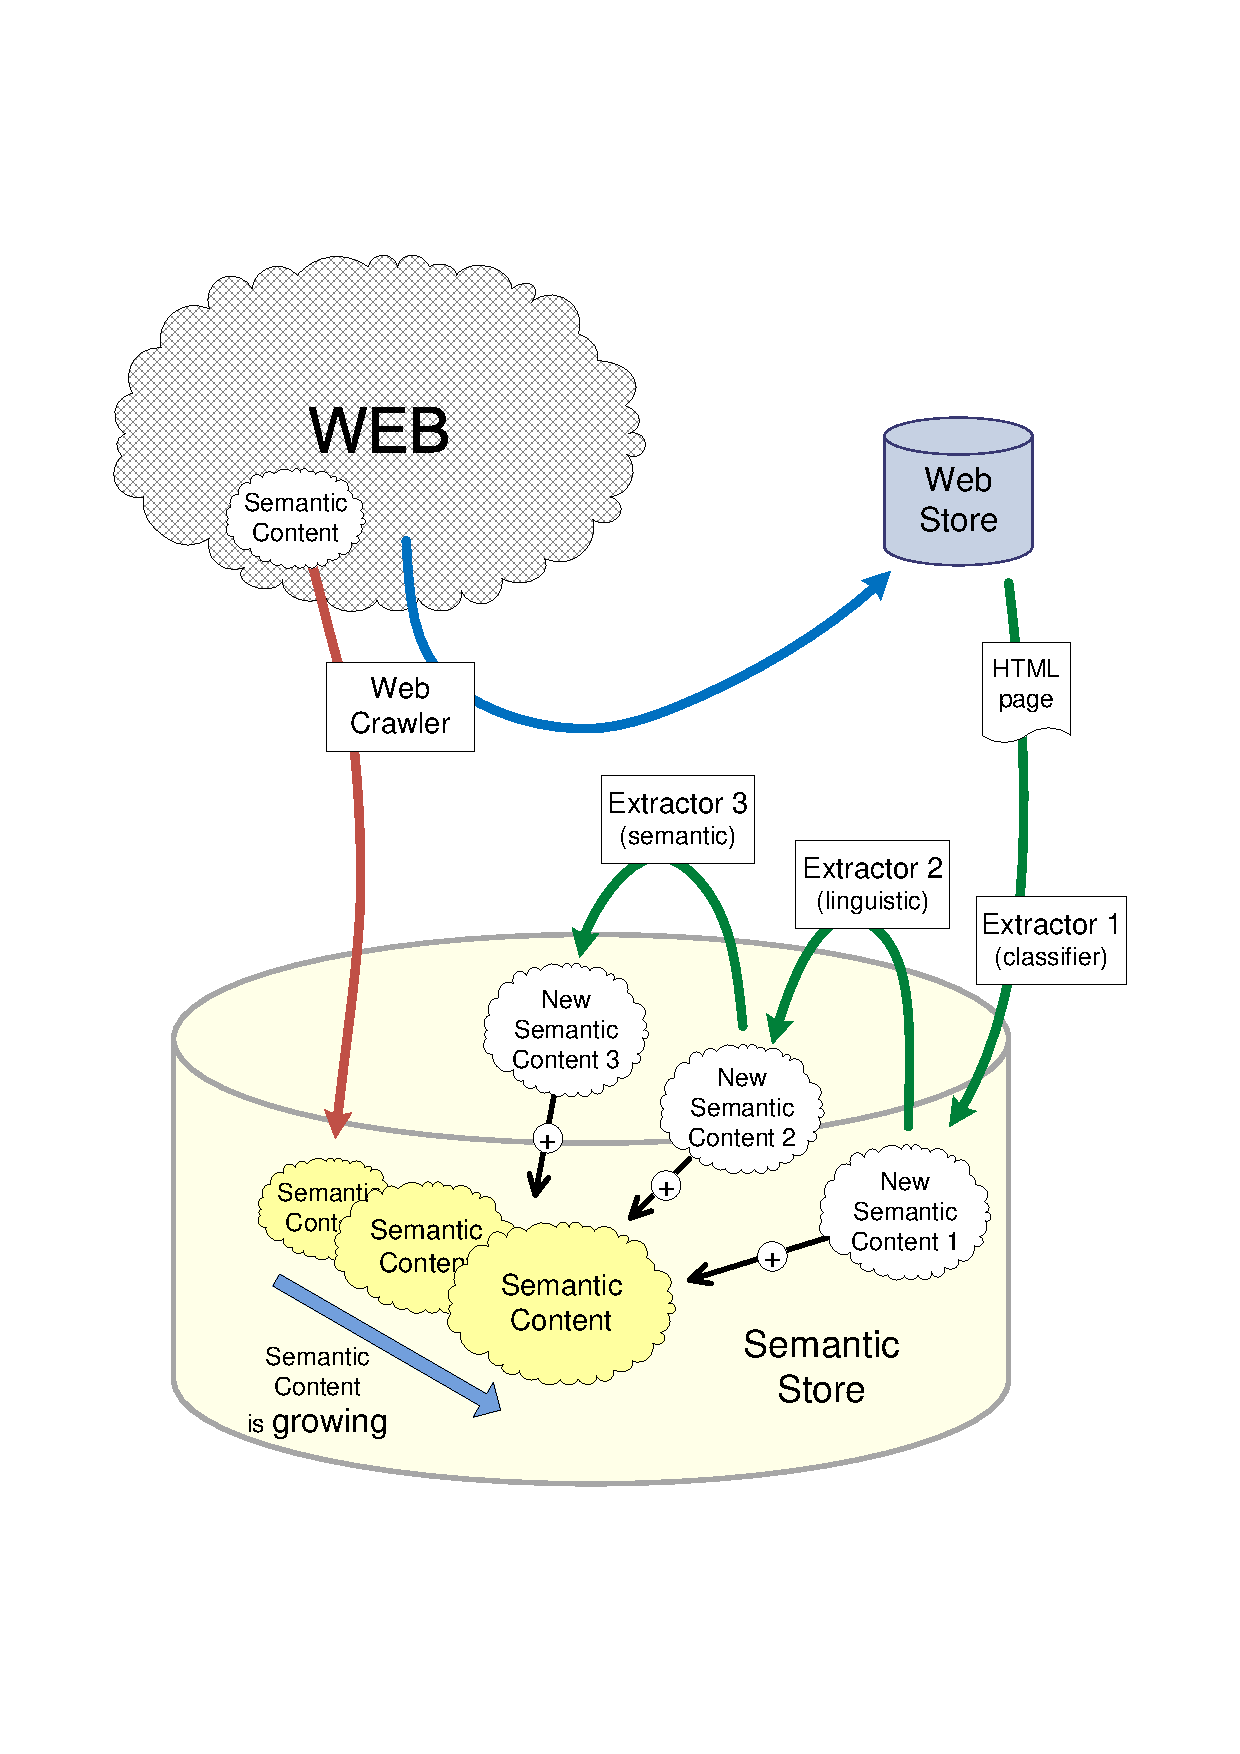
\includegraphics[height=.85\hsize, width=\hsize]{img/Semantization}
\caption{The process of semantization of the Web}
\label{img:Semantization}
\end{figure}


%In their Scientific American 2001 article \cite{biblio:2001-Berners-Lee-SemanticWeb}, Tim Berners-Lee, James Hendler and Ora Lassila unveiled a nascent vision of the semantic web: a highly interconnected network of data that could be easily accessed and understood by a desktop or handheld machine. They painted a future of intelligent software agents that would ``answer to a particular question without our having to search for information or pore through results'' (quoted from \cite{biblio:feigenbaum_semantic_2007}).
Recently, Lee Feigenbaum, Ivan Herman, Tonya Hongsermeier, Eric Neumann and Susie Stephens in their Scientific American 2007 article \cite{biblio:feigenbaum_semantic_2007} conclude that ``Grand visions rarely progress exactly as planned, but the Semantic Web is indeed emerging and is making online information more useful as ever''. They support their claim with success of semantic web technology in drug discovery and health care (and several other applications). By our opinion, these are mainly corporate applications with data annotated by humans.

Ben Adida when bridging clickable and Semantic Web with RDFa (\cite{biblio:AdidaClickable}) assumes also human (assisted) activity - annotations of newly created web resources. \par

What to do with the content of the web of today or of pages published without annotations? The content of the web of today is too valuable to be lost for emerging semantic web applications. We are looking for a solution how to make it accessible in semantic manner. \par

We would like to address the problem of semantization (enrichment) of current web content as an automated process of third party annotation for making at least a part of today's web more suitable for machine processing. It would hence allow intelligent tools to search and recommend things on the web (as advocated by Tim Berners-Lee \cite{biblio:LeeWebThings}). Our approach is not limited only to one specific domain of application, it can be used across all the disciplines presented on the web. Fro example in \cite{biblio:eEnvi} we have demonstrated how our approach can help with environmental issues.



\section{Prototypes and experiments}

Our main idea is to fill a semantic repository with information that is automatically extracted from the web and make it available to software agents. We are working on a proof of concept that this idea is realizable and we give results of several experiments in this direction.

Our web crawler (see Fig.\ref{img:Semantization})
downloads a part of the web to the web repository (web archive). 
%Resources with semantic content can be uploaded directly to the semantic repository (Semantic Store). 
Page classifier selects those parts of web archive which are suitable for further semantic enrichment (we are able to enrich only a part of resources). More semantic content is created by several extractors and annotators in several phases. %The emphasis of this paper is on the automation and the usage of such extracted/enriched data.


%Here we would like to present the idea of our contribution to web semantization.

\textbf{(1) The idea of a web repository.}  

%We decided to enrich only textual content for the present, no multimedia (this substantially reduces the size of information we have to store). Especially we restrict to the pages with content consisting either dominantly of grammatical sentences (let us call them textual pages) and those containing large number of table cells (let us call them tabular pages). Of course this division need not be disjoint, and will not cover the whole web. 


%\subsection{Web repository}
The web repository is a temporal repository of web documents crawled by a crawler. The repository supports document's metadata, e.g. modification and creation dates, domain name, ratio of HTML code/text, content type, language, grammatical sentences etc. It keeps track of all changes in a document and simplifies access to and further processing of Web documents. We are experimenting with the web crawler Egothor\footnote{http://www.egothor.org/} 2.x and it's web repository. %We have filled this repository with several terabytes of textual part of Czech web (domain *.cz) and it very simplified access to this data. {\bf je mozne podstatne skratit}
For pages from hidden web we have used RSS feeds.

%The architecture is based on three layers: core that saves documents and computes deltas between revisions to save space; symlink that maps core's document and revision numbers to numbers published to a user; cloud that assigns tags and manages ACL on the tags. This way the system can modify the tags without overloading the main base of raw documents.

%, so that it is able to provide information about a durable (persistent) text blocks or even subtrees in DOM.


%To be able to separate durable grammatical or table pages poses special requirements to search in our web repository.\par

\textbf{(2) The second idea is to split annotation process into two parts}, the first is domain independent intermediate annotation and the second is domain dependent user directed annotation of a smaller portion of the web. Semantic enrichment is in fact a data mining task (although a special one) - to add to web documents a piece of knowledge, which is obvious for human perception and hard for a machine. That means to annotate data by concepts from an ontology which is the same as to map instances to ontology. Such a data mining task will be easier to solve when there is a sort of a repetition (modulo some similarity).\par 
Both annotation tasks should be automated, with some initial human assisted learning. The first part of learning could require assistance of a highly skilled expert; the second (probably faster part) should be doable by an user with average computer literacy. \par

%The first domain independent annotation will serve as an intermediate annotation supporting further processing. This will run once on the whole suitable data. Hence initial necessary human assistance in training can be done by a highly skilled expert (indeed it can be a longer process).\par

%The second domain dependent annotation part can consists of a large number of tasks with different domains and ontologies. This should be possible to be executed very fast and if possible with assistance of an average computer skilled user.  We can afford this having intermediate annotation. \par

%\begin{figure}[b!]
%\centering
%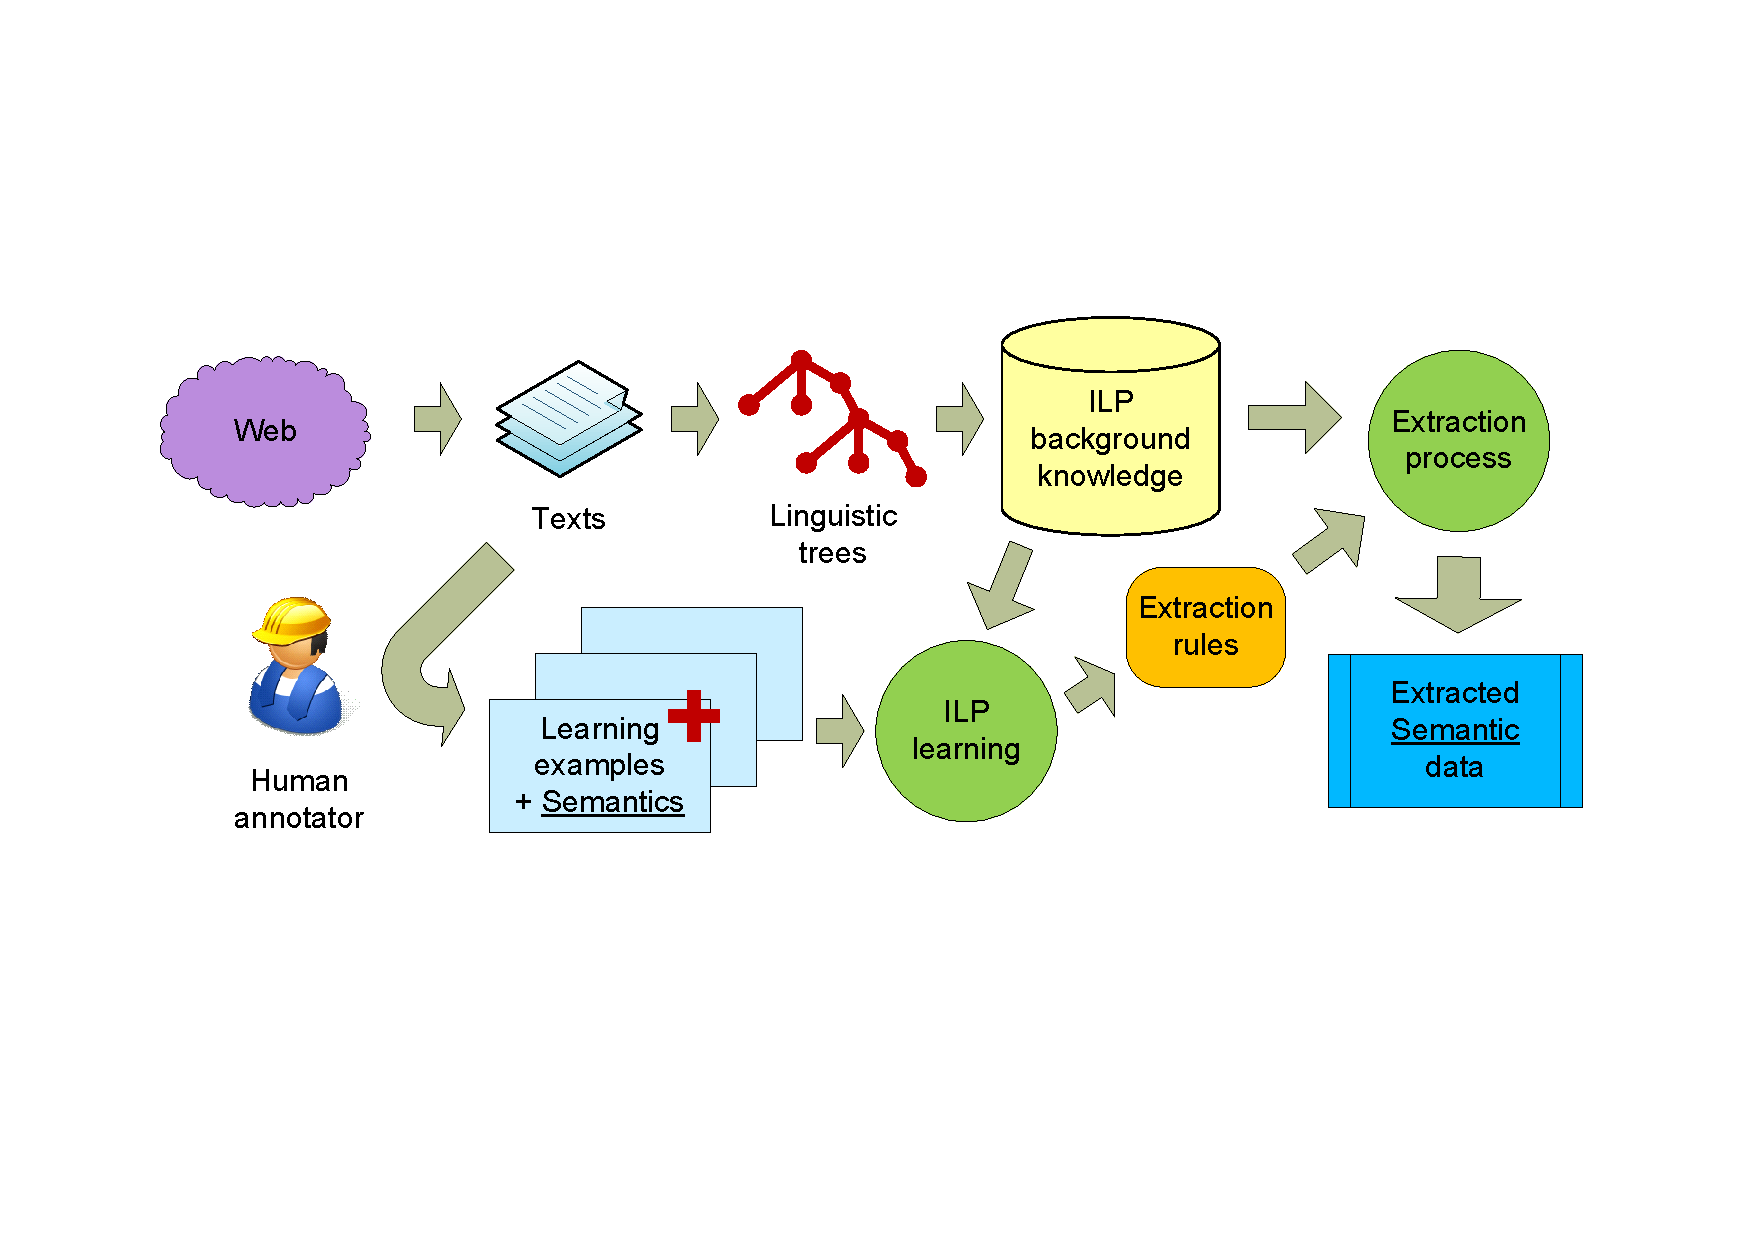
\includegraphics[width=\hsize]{img/DedVoj_ILP}
%\caption{ILP Learning of Extraction Rules}
%\label{img:DedVoj_ILP}
%\end{figure}



\textbf{Domain independent intermediate annotation} can be done with respect to general ontologies. We distinguish two cases: (1) textual resources and (2) structured resources. For \emph{textual resources} the ontology we use is the general linguistic PDT tectogrammatical structure \cite{biblio:zkraceno_MiBeAnnotationtectogrammatical2006} which captures semantic meaning of grammatical sentences in Czech. 
%This is the task for computational linguistics; we make use of their achievements which were originally focused on machine translation.
For example English language can be parsed in many different ways (most often according to some kind of grammar). {\bf Current solution} makes use of a tree structure of the annotations. In this paper we will present our experience with Czech language and tectogrammatical structure that we have used for domain independent intermediate annotation of pages dominantly consisting of grammatical sentences. 

%\newline
%\texttt{\phantom{mmm}\_:sentence dev:text "Nobody was injured.".\\
%\phantom{mmm}\_:sentence pdt:t\_lemma "injured".\\
%\phantom{mmm}\_:sentence pdt:negation true.}


For \emph{structured survey or product summary pages} we assume that their structure is often similar and the common structure can help us to detect data regions and data records and possibly also attributes and their values from detailed product pages. Annotation tools will be trained by humans here also -- nevertheless only once for the annotation of the whole repository. {\bf Current solution} uses similarities of DOM structure of pages.

% We use ontology which denotes data regions and data records, see below.
%\newline
%\texttt{\phantom{mmm}URL dev:hasDataRegion \_:DReg1.\\
%\phantom{mmm}\_:DReg1 dev:startsAt \emph{nodeInTheDOMofURL}.\\
%\phantom{mmm}\_:DReg1 dev:endsAt \emph{nodeInTheDOMofURL}.}

%We have identified two types of web resources where this can be done. The first are "table pages", containing large number of cells with abbreviated description of a resource and corresponding detailed pages. Here we assume that content of cells is similar and content of detailed pages is also similar. Because of space limitations, we do not describe our approach for these pages.

%The second are pages dominantly consisting of grammatical sentences. Thanks to the fact that we have a third party linguistic tool for the creation of tectogrammatical trees of sentences, this can be done without requirement of similarity repetition. This situation is illustrated in the Fig.~\ref{fig:similarity}.

%We can see an interesting inversion in the use of similarity and repetition. %depicted in Fig.~\ref{fig:similarity}.

%While for tabular pages we use similarities in the intermediate phase, for textual pages we use similarities in the domain dependent phase where similar sentences often occur.


%\begin{figure}
%\label{fig:similarity}
%\begin{center}
%\begin{tabular}{|p{100pt}||p{100pt}|p{100pt}|} \hline
%Type of annotation&Tabular pages&Textual pages\\ \hline\hline
%Intermediate general&Uses similarities&Does not use similarities\\ \hline
%Domain dependent&Does not use similarities&Uses similarities\\ \hline
%\end{tabular}	
%\end{center}
%\caption{Use of similarity in annotation approaches}
%\end{figure} 

\textbf{Domain dependent annotation} is concerning only pages previously annotated by general ontologies. This makes second annotation faster and easier. An assistance of a unskilled human is assumed here for each domain and a new ontology. Nevertheless we cannot expect an average user to annotate a big amount of resources, so we have to work with the realistic (30 to 40) size of test set.

Repetitions in \emph{textual pages} make possible to learn a mapping from structured tectogrammatical instances to an ontology. %This domain (task) dependent task can be avoided by a collaborative filtering method, assuming there is enough users' acquaintance. \par
{\bf Current solution} uses ILP tool \texttt{PROGOL} over annotations obtained in the first domain independent part.
%It is demonstrated in Fig.~\ref{img:DedVoj_ILP}.
For traffic accident reports, we were able to learn rules for finding sentences reporting on injuries (note that linguistic is need in sentences like 'nobody was injured', simple key word search does not work in this case) 

\noindent\texttt{Rule set1:\\
injured(A):-edge(A,C),edge(C,D),t\_lemma(D,accident).\\
injured(A):-edge(A,C),t\_lemma(A,injure),neg(C,false).}

See \texttt{Rule set1} as an example of learned rules. Fig.~\ref{fig:results} shows the 4-fold table where rows depict classification by rule set and columns classification by user. Results are promising, nevertheless tagging is done by unskilled user for whom the tagging is usually tedious.

For \emph{structured pages} the domain dependent annotation \textbf{current solution} uses simple ontology in a form of relational schema provided by user. We experiment with several heuristics for learning regular expressions for attribute values.

\begin{figure}
\label{fig:results}
\centering
\begin{tabular}{|c|c|c|} \hline
 		&User tag	&$\neg$User	tag\\ \hline
Rule set1		& 11&1 \\ \hline
$\neg$Rule set1	& 4 &22\\ \hline
\end{tabular}
\caption{Results on the realistic test set}
\end{figure}


\textbf{(3) Next idea is to design a semantic repository}. It should store all the semantic data extracted by extraction tools and accessed through a semantic search engine. 
%Of course many different problems (e.g. querying and scalability) are connected with this but they are at least partially solved now days. 
{\bf Current solution} uses \cite{biblio:DoTySemanticWeb2007}. It supports RDF storage and SPARQL querying.

%The semantic repository should also contain some sort of uncertainty annotation besides other ontologies. The main reason is that annotation process is error prone and we can have in future different alternative annotation tools and aggregate results. This aspect is not further described in the paper but can be found with many details in \cite{biblio:DeEcDiscussionUncertainty2008}. %and \cite{biblio:EcHoUncertaintyIssues2008}.\par

\textbf{(4) Design of an software agent}, which will give the evidence that our semantization really improved general web search. Besides using annotated data it should also contain some user dependent preference search capabilities. %{\bf radsi citovat neco o uceni preferenci nez o neurcitosti}. 
{\bf Current solution} exploits user preference modelling technique published in our previous work \cite{biblio:EcHoLearningdifferent2007}.



\begin{figure}
\centering
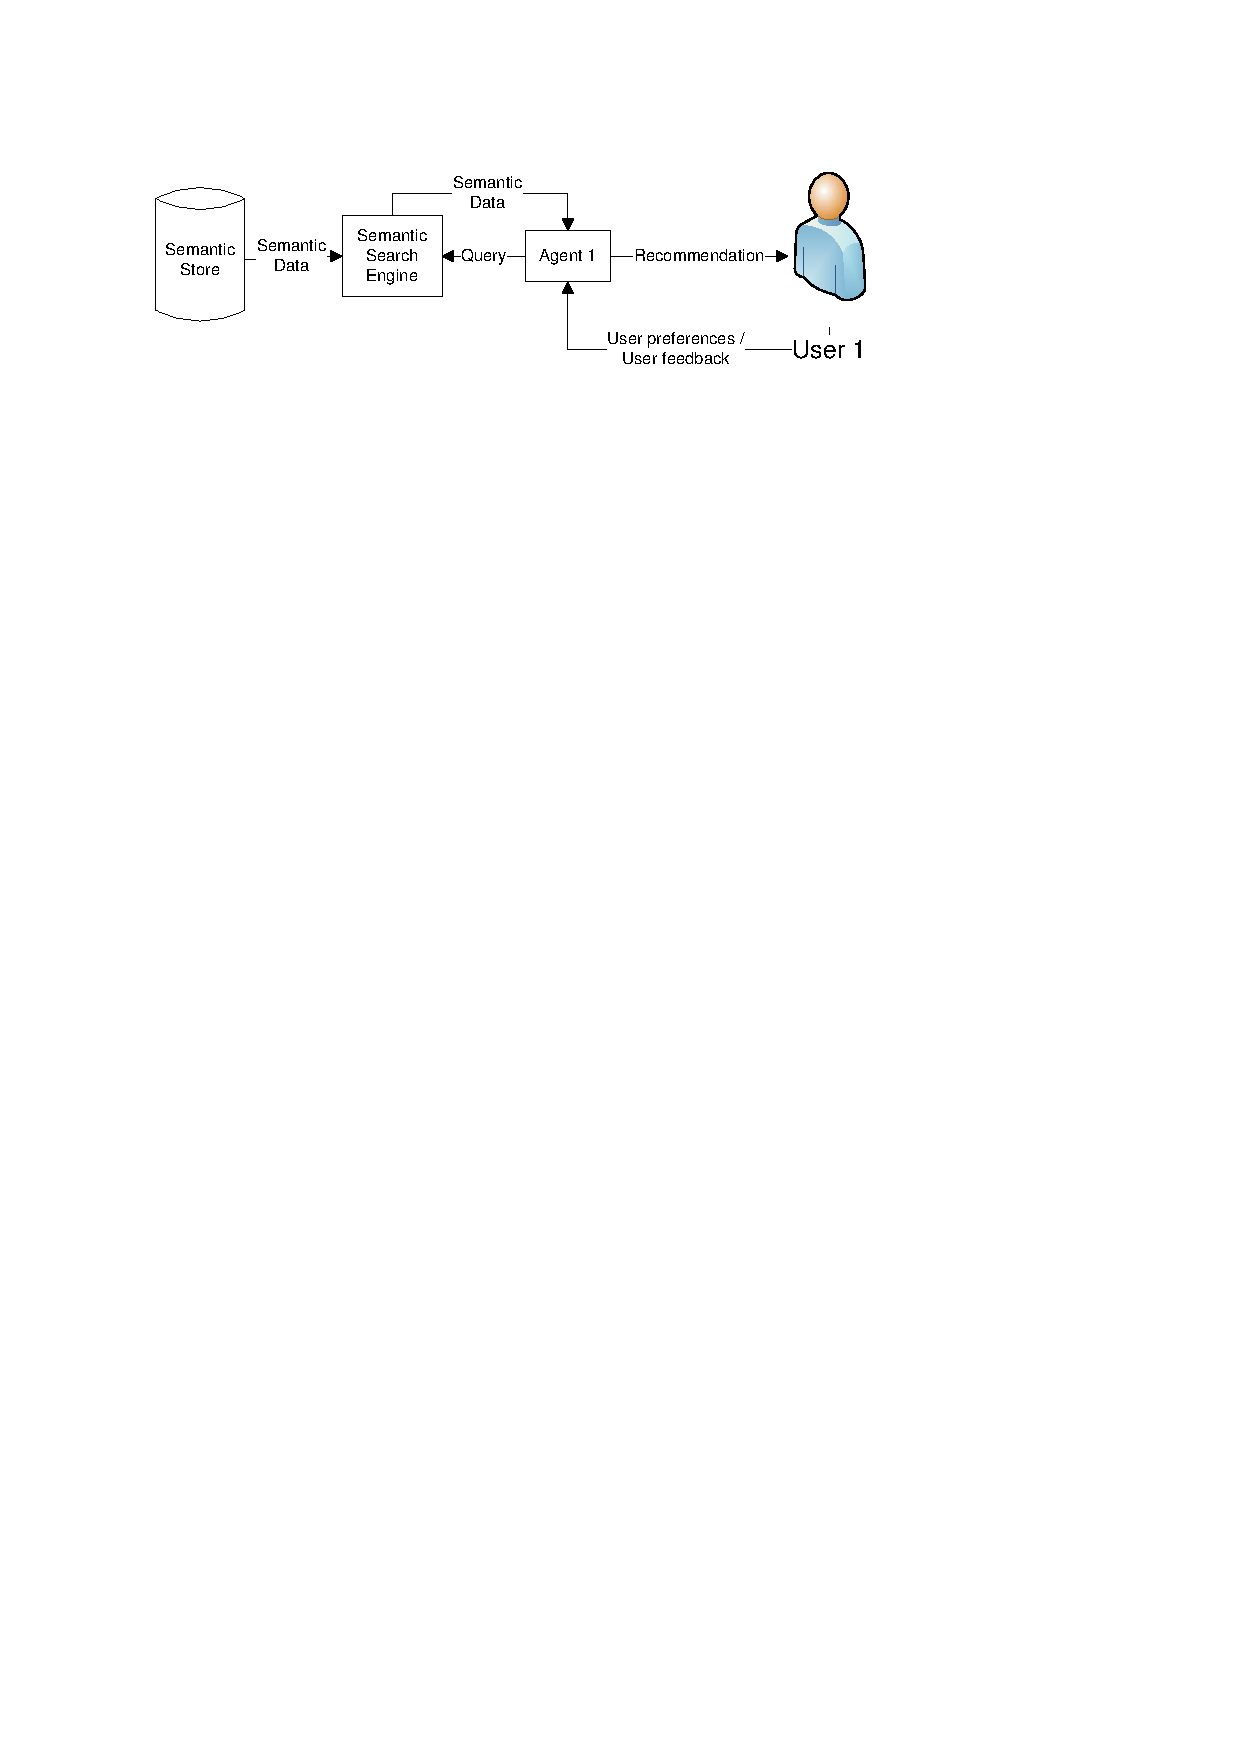
\includegraphics[width=\hsize, height=.3\hsize]{img/UserSearch}
%\caption{Process of querying Semantic Search Engine by an user agent}
\caption{Querying Semantic Search Engine}
\label{img:UserSearch}
\end{figure}
 
The process of a user agent searching and making use of semantic search engine is represented in Figure \ref{img:UserSearch}.

%Our main focus in this paper is on the agent and on the extractors.


%\begin{figure}
%\centering
%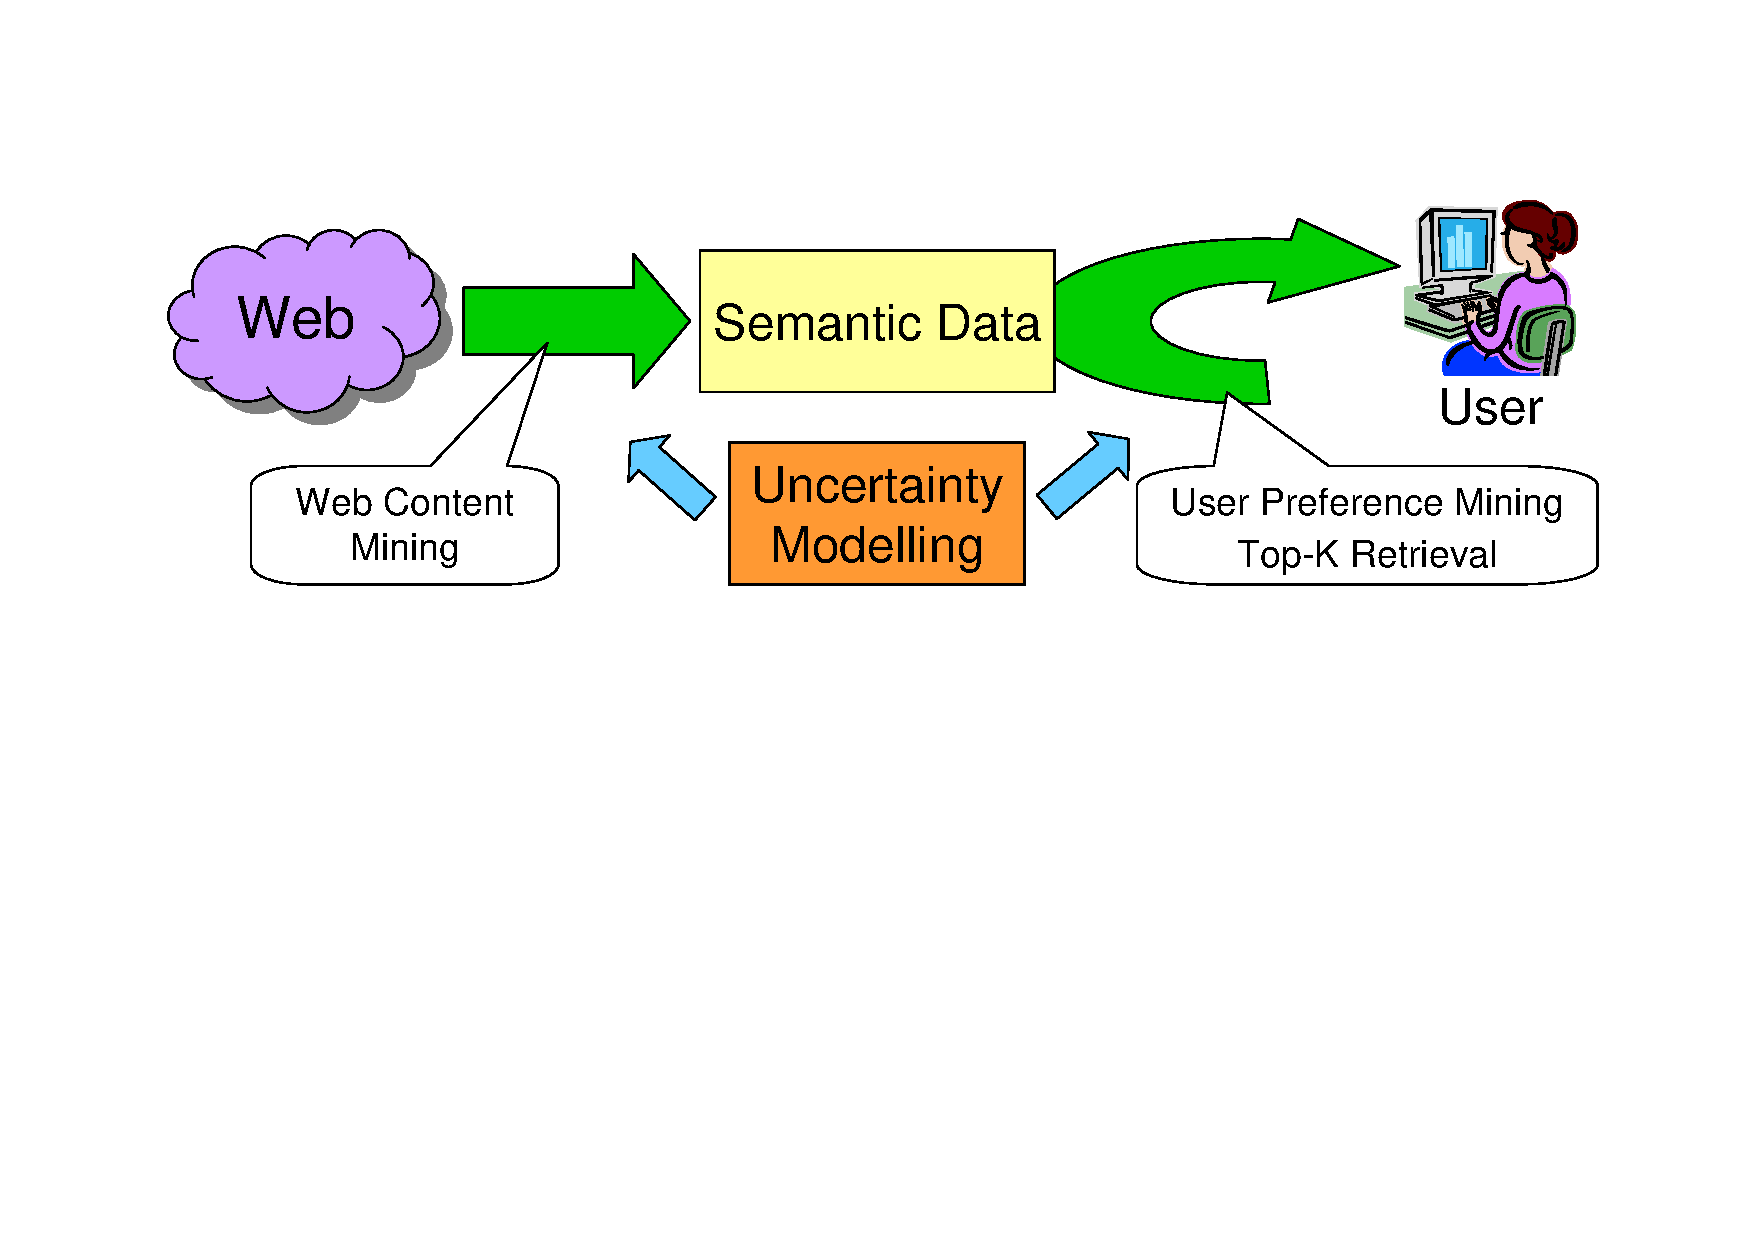
\includegraphics[width=\hsize]{img/Web2User}
%\caption{Connecting Web and User}
%\label{img:Web2User}
%\end{figure}

%\begin{figure}
%\centering
%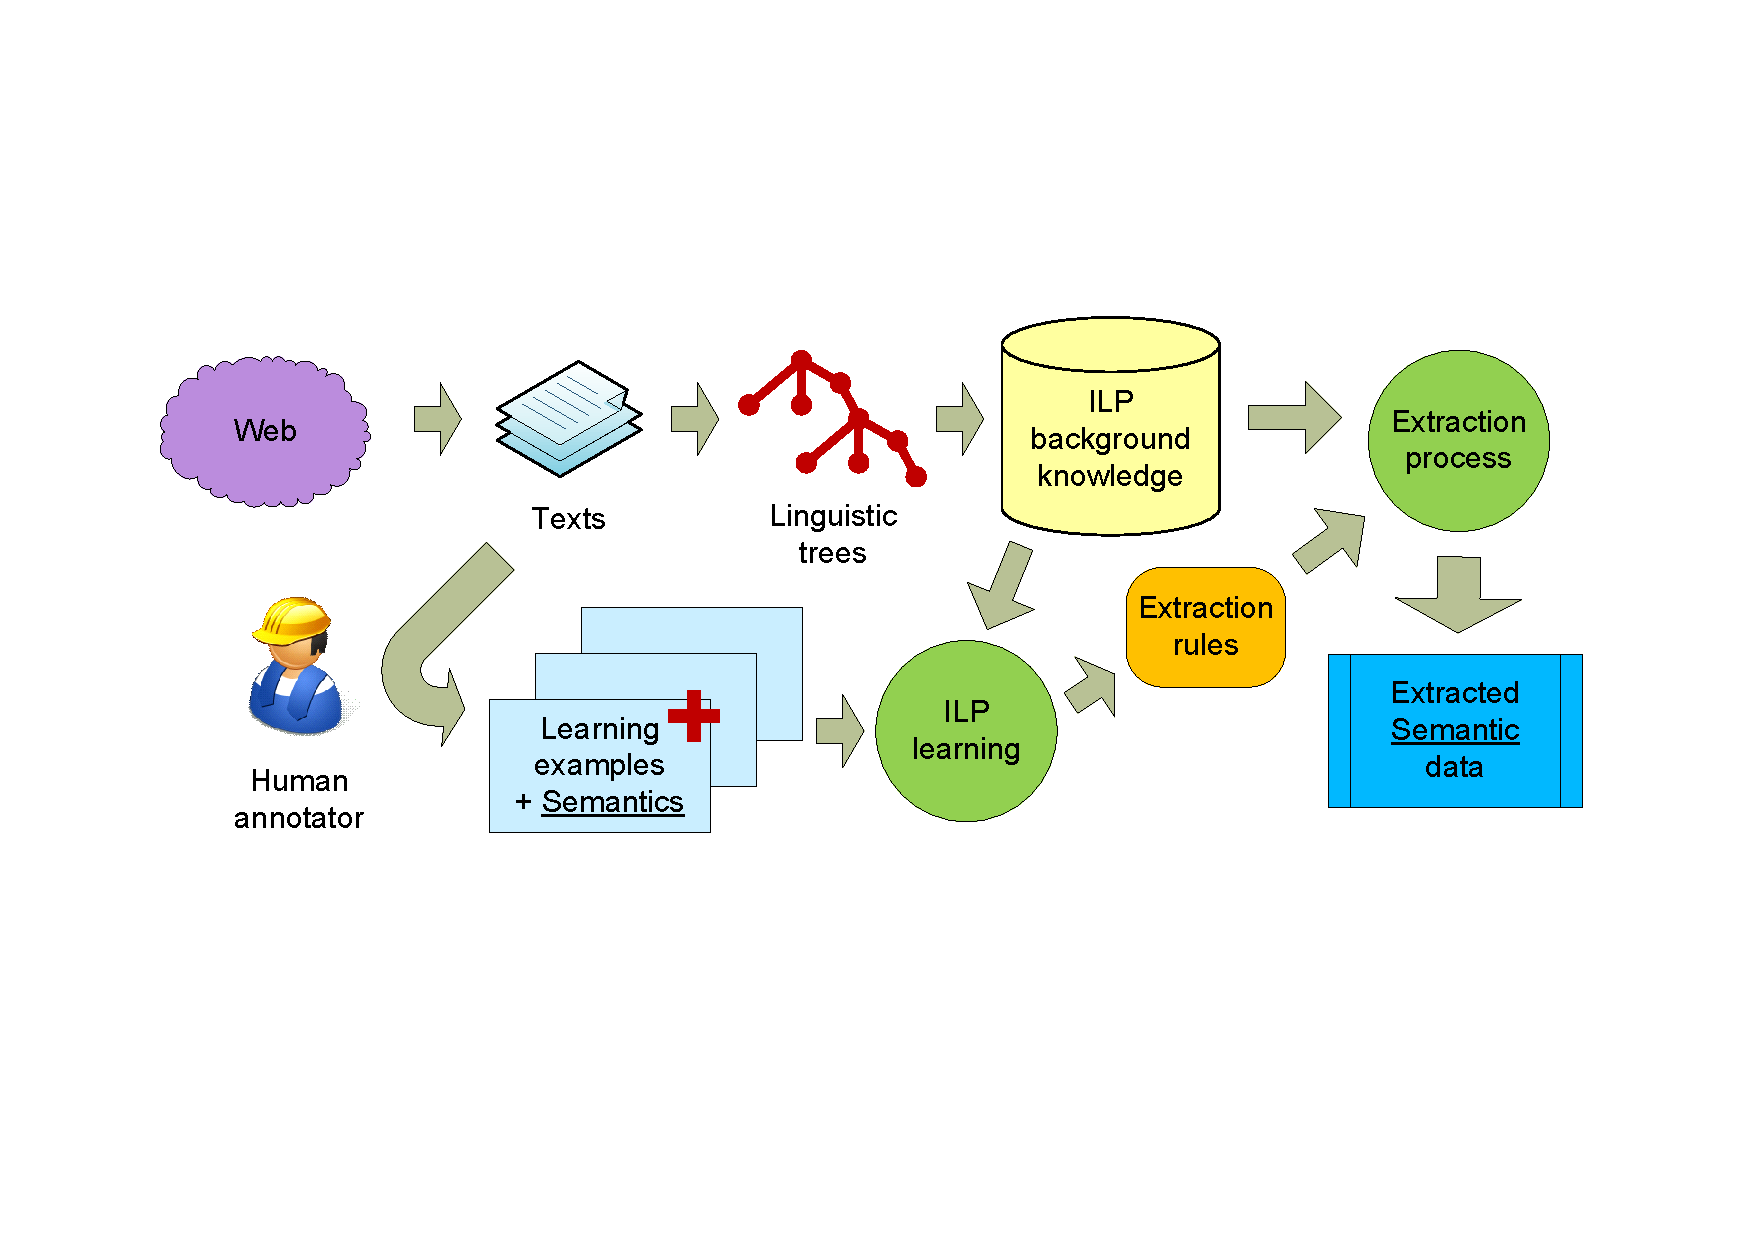
\includegraphics[width=\hsize]{img/DedVoj_ILP}
%\caption{ILP Learning of Extraction Rules}
%\label{img:DedVoj_ILP}
%\end{figure}

%ACKNOWLEDGMENTS are optional
\section{Conclusion}
In this paper we have presented our work on web semantization -- models and prototypes making the web to the web of things (\cite{biblio:LeeWebThings}). Preliminary experiments are promising.
%\section{Acknowledgments}

This work was partially supported by Czech projects\\1ET100300517, 201/09/0990 GACR and MSM-0021620838.

%
% The following two commands are all you need in the
% initial runs of your .tex file to
% produce the bibliography for the citations in your paper.
\bibliographystyle{abbrv}
\bibliography{DedEckVoj_FET09}

\balancecolumns % GM July 2000
% That's all folks!
\end{document}
